\documentclass{standalone}
\usepackage[T1]{fontenc}
\usepackage{siunitx}
\usepackage{tikz}

\usetikzlibrary[arrows,positioning,matrix]

\begin{document}
\begin{tikzpicture}
  \node[draw=none] (example) {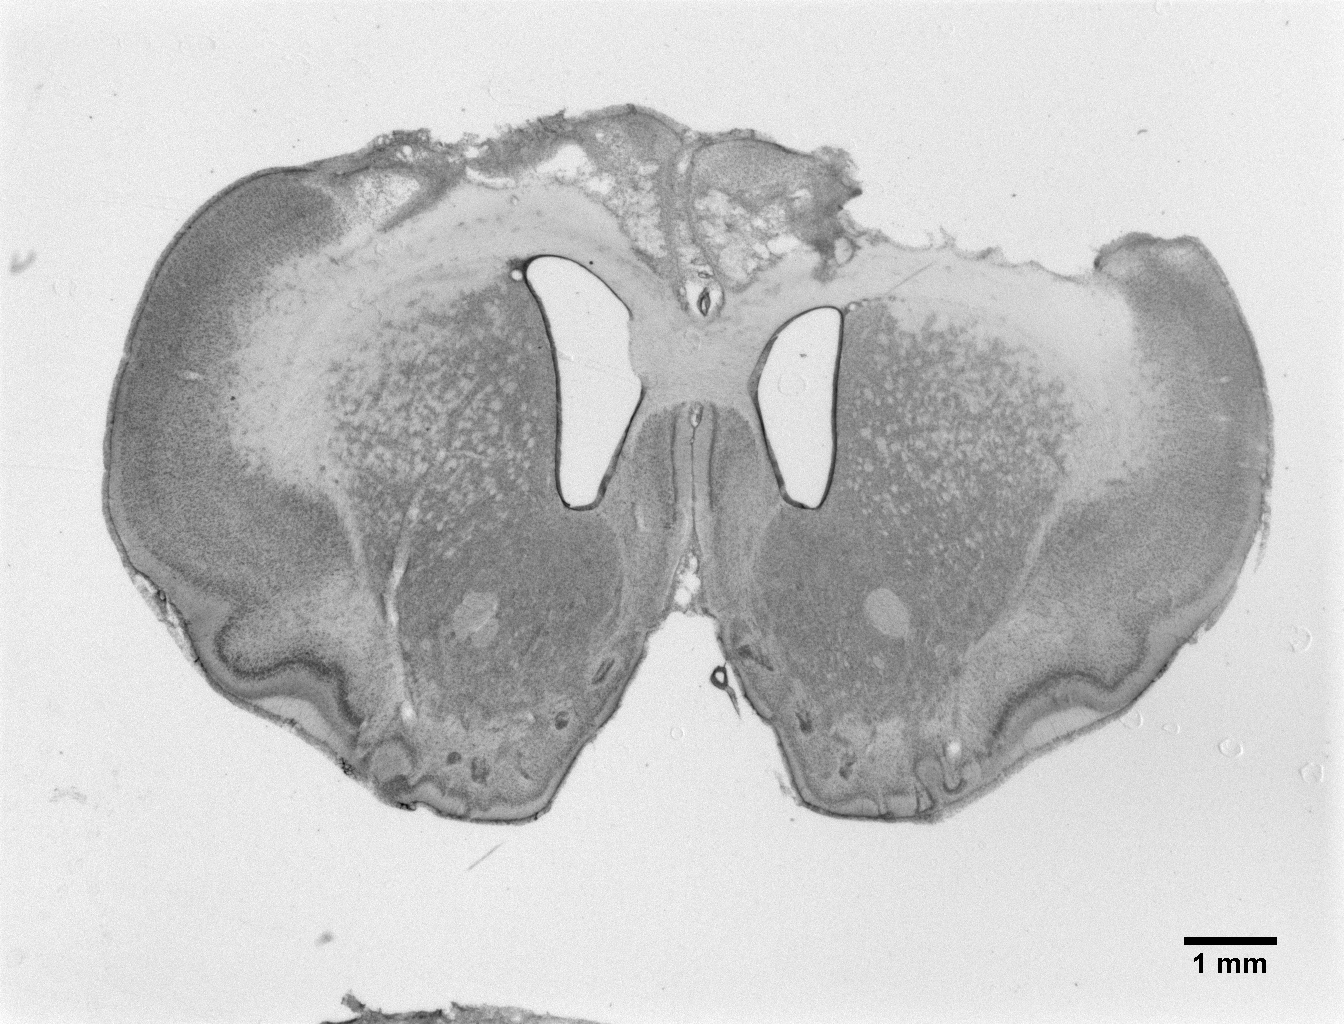
\includegraphics[width=0.5\textwidth]{elements/lesionA_viewplate_bregma228-slice33}};
  \node[draw=none,above left=0mm of example] {A};
  \node[draw=none,below right=-5.4cm and 3.5mm of example] (volumes) {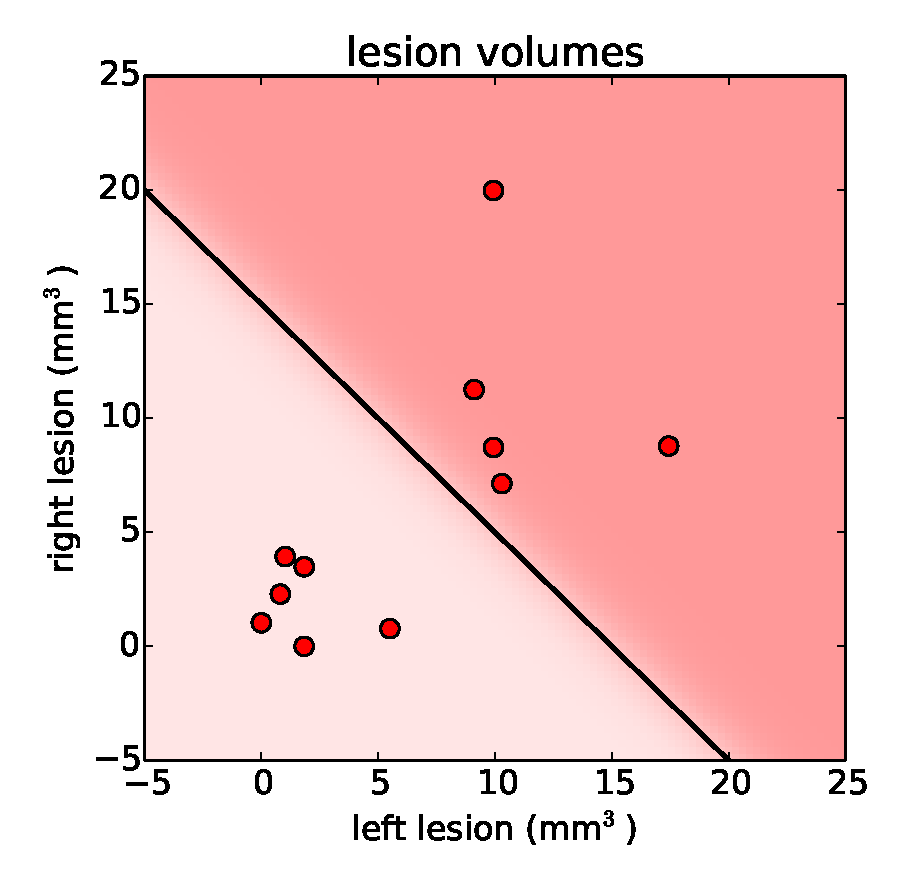
\includegraphics[width=0.5\textwidth]{elements/lesionvolumes}};
  \node[draw=none,above right=0mm and 2mm of example] {B};
  \node[draw=none,below=1.5cm of example] (small) {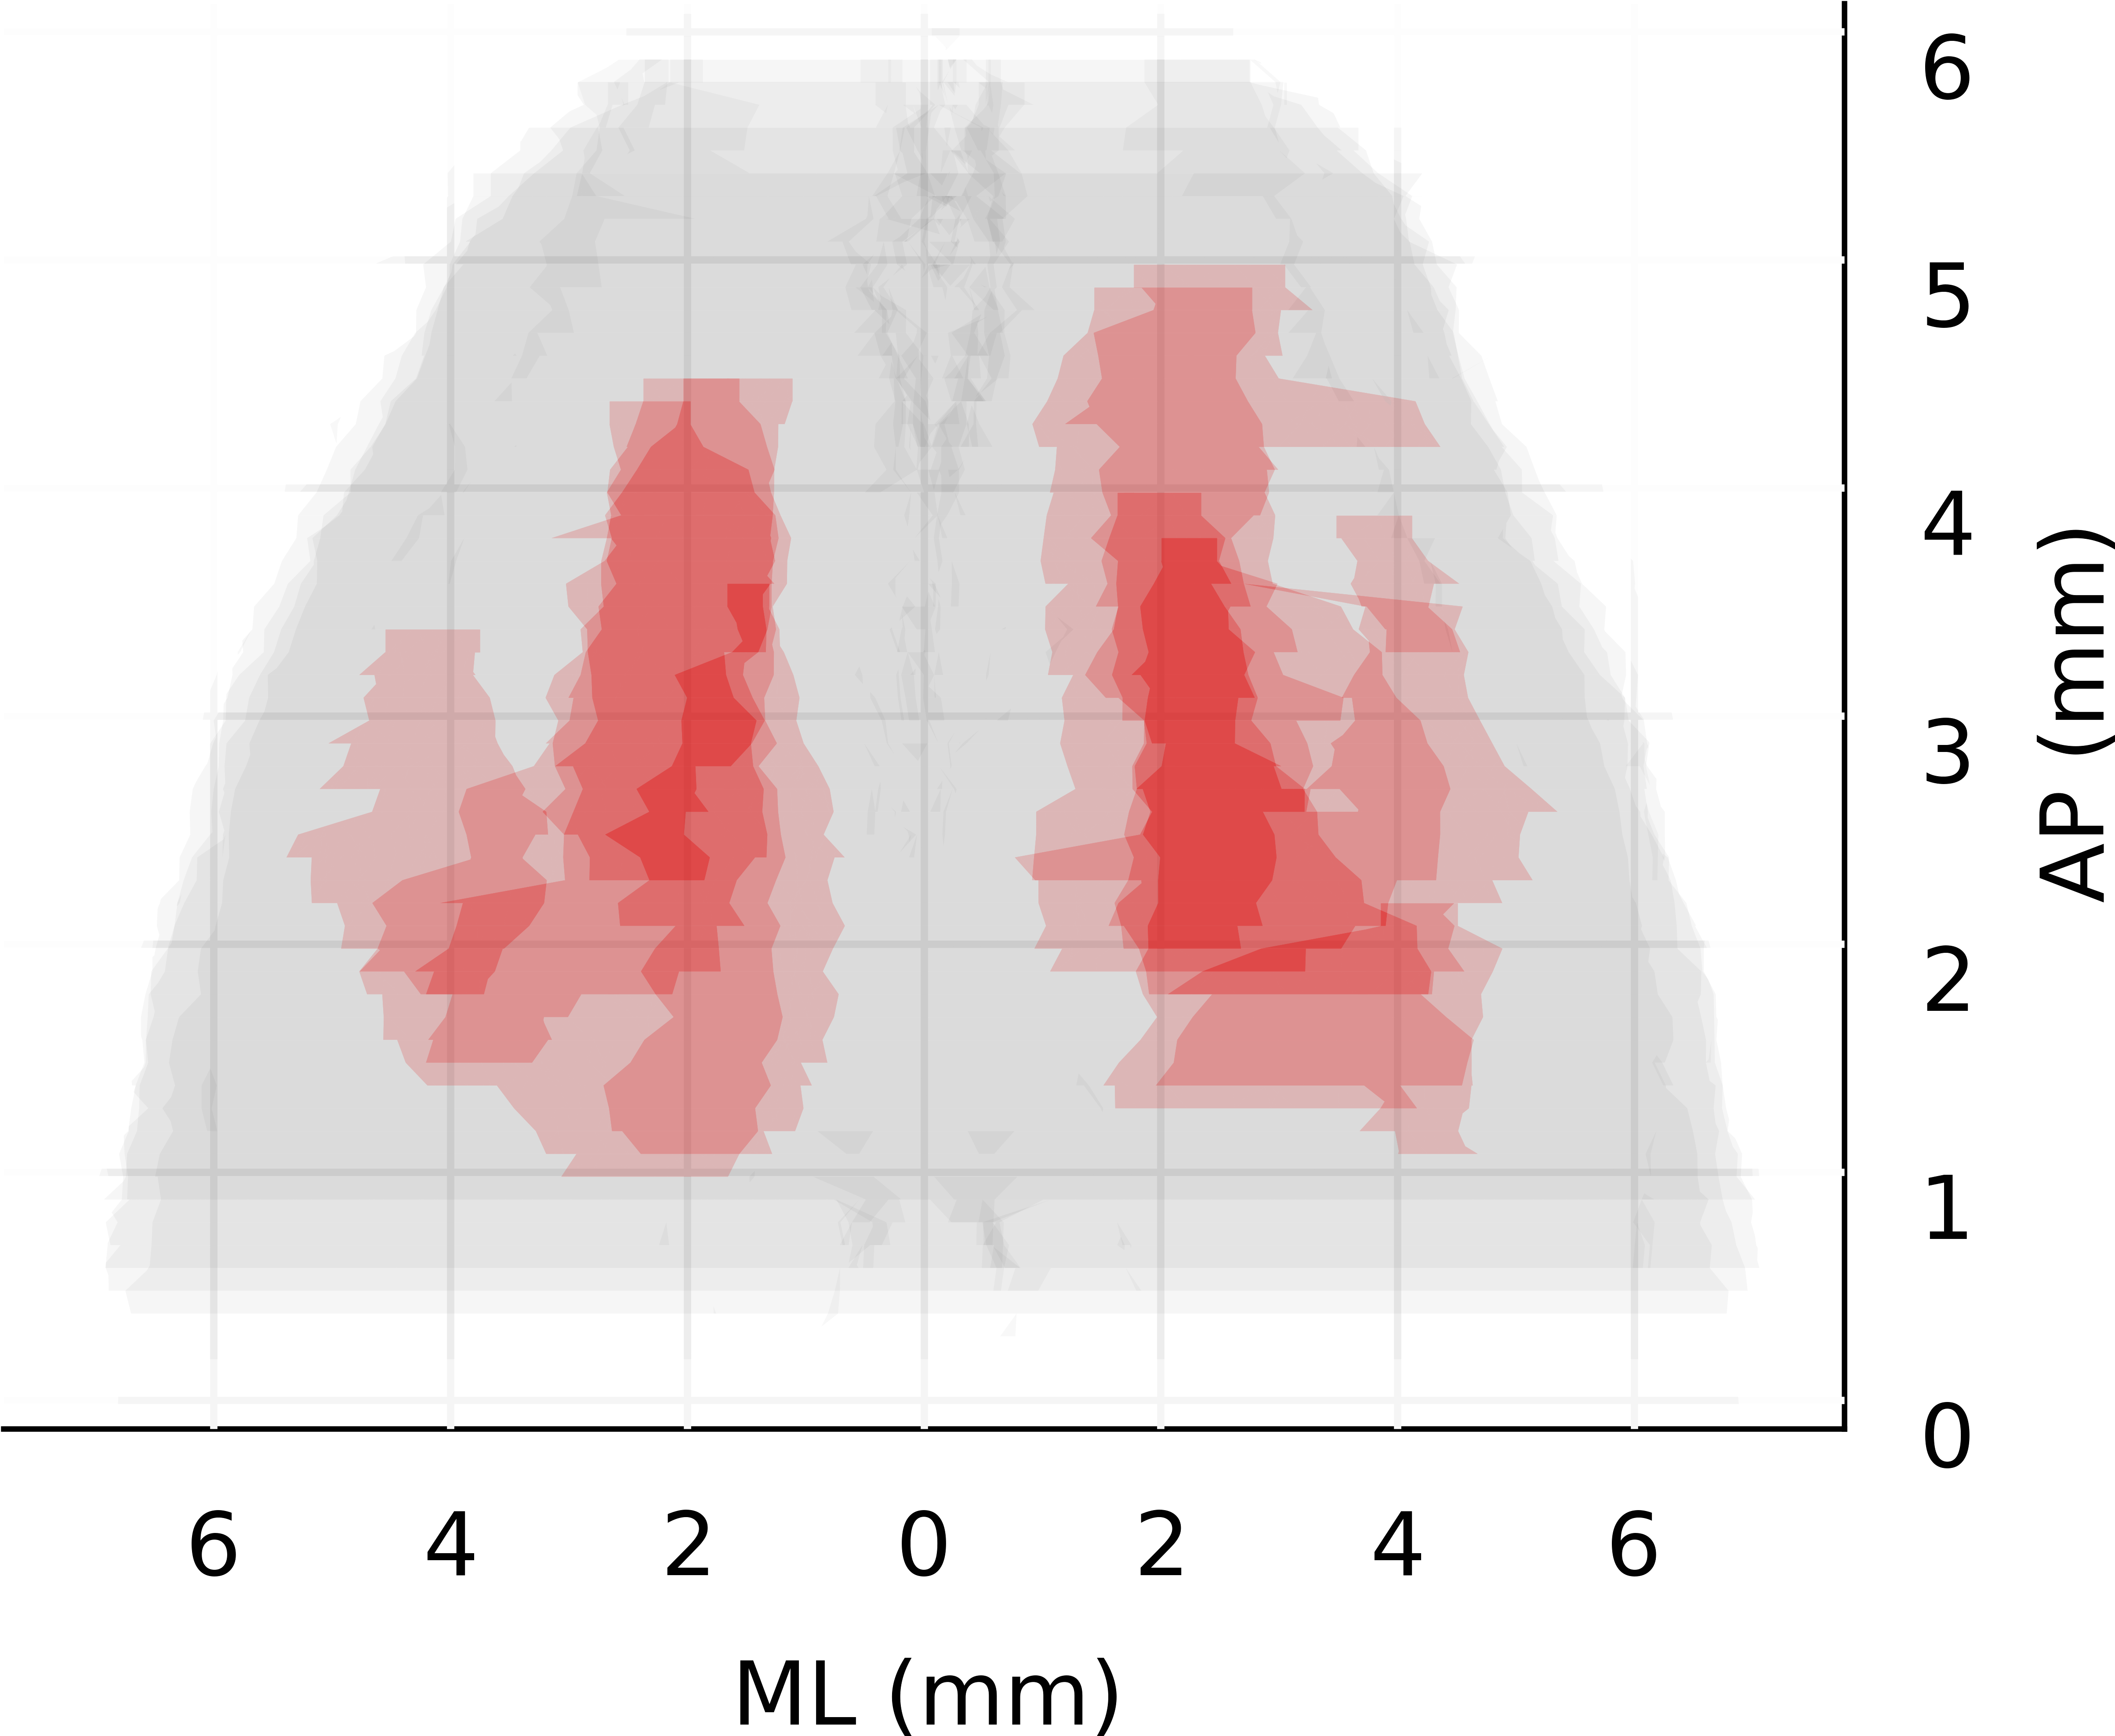
\includegraphics[width=0.5\textwidth]{elements/histology_small}};
  \node[draw=none,above=0mm of small] {small lesions (< \SI{15}{\milli\meter\cubed})};
  \node[draw=none,above left=5mm and 0mm of small] {C};
  \node[draw=none,right=of small] (large) {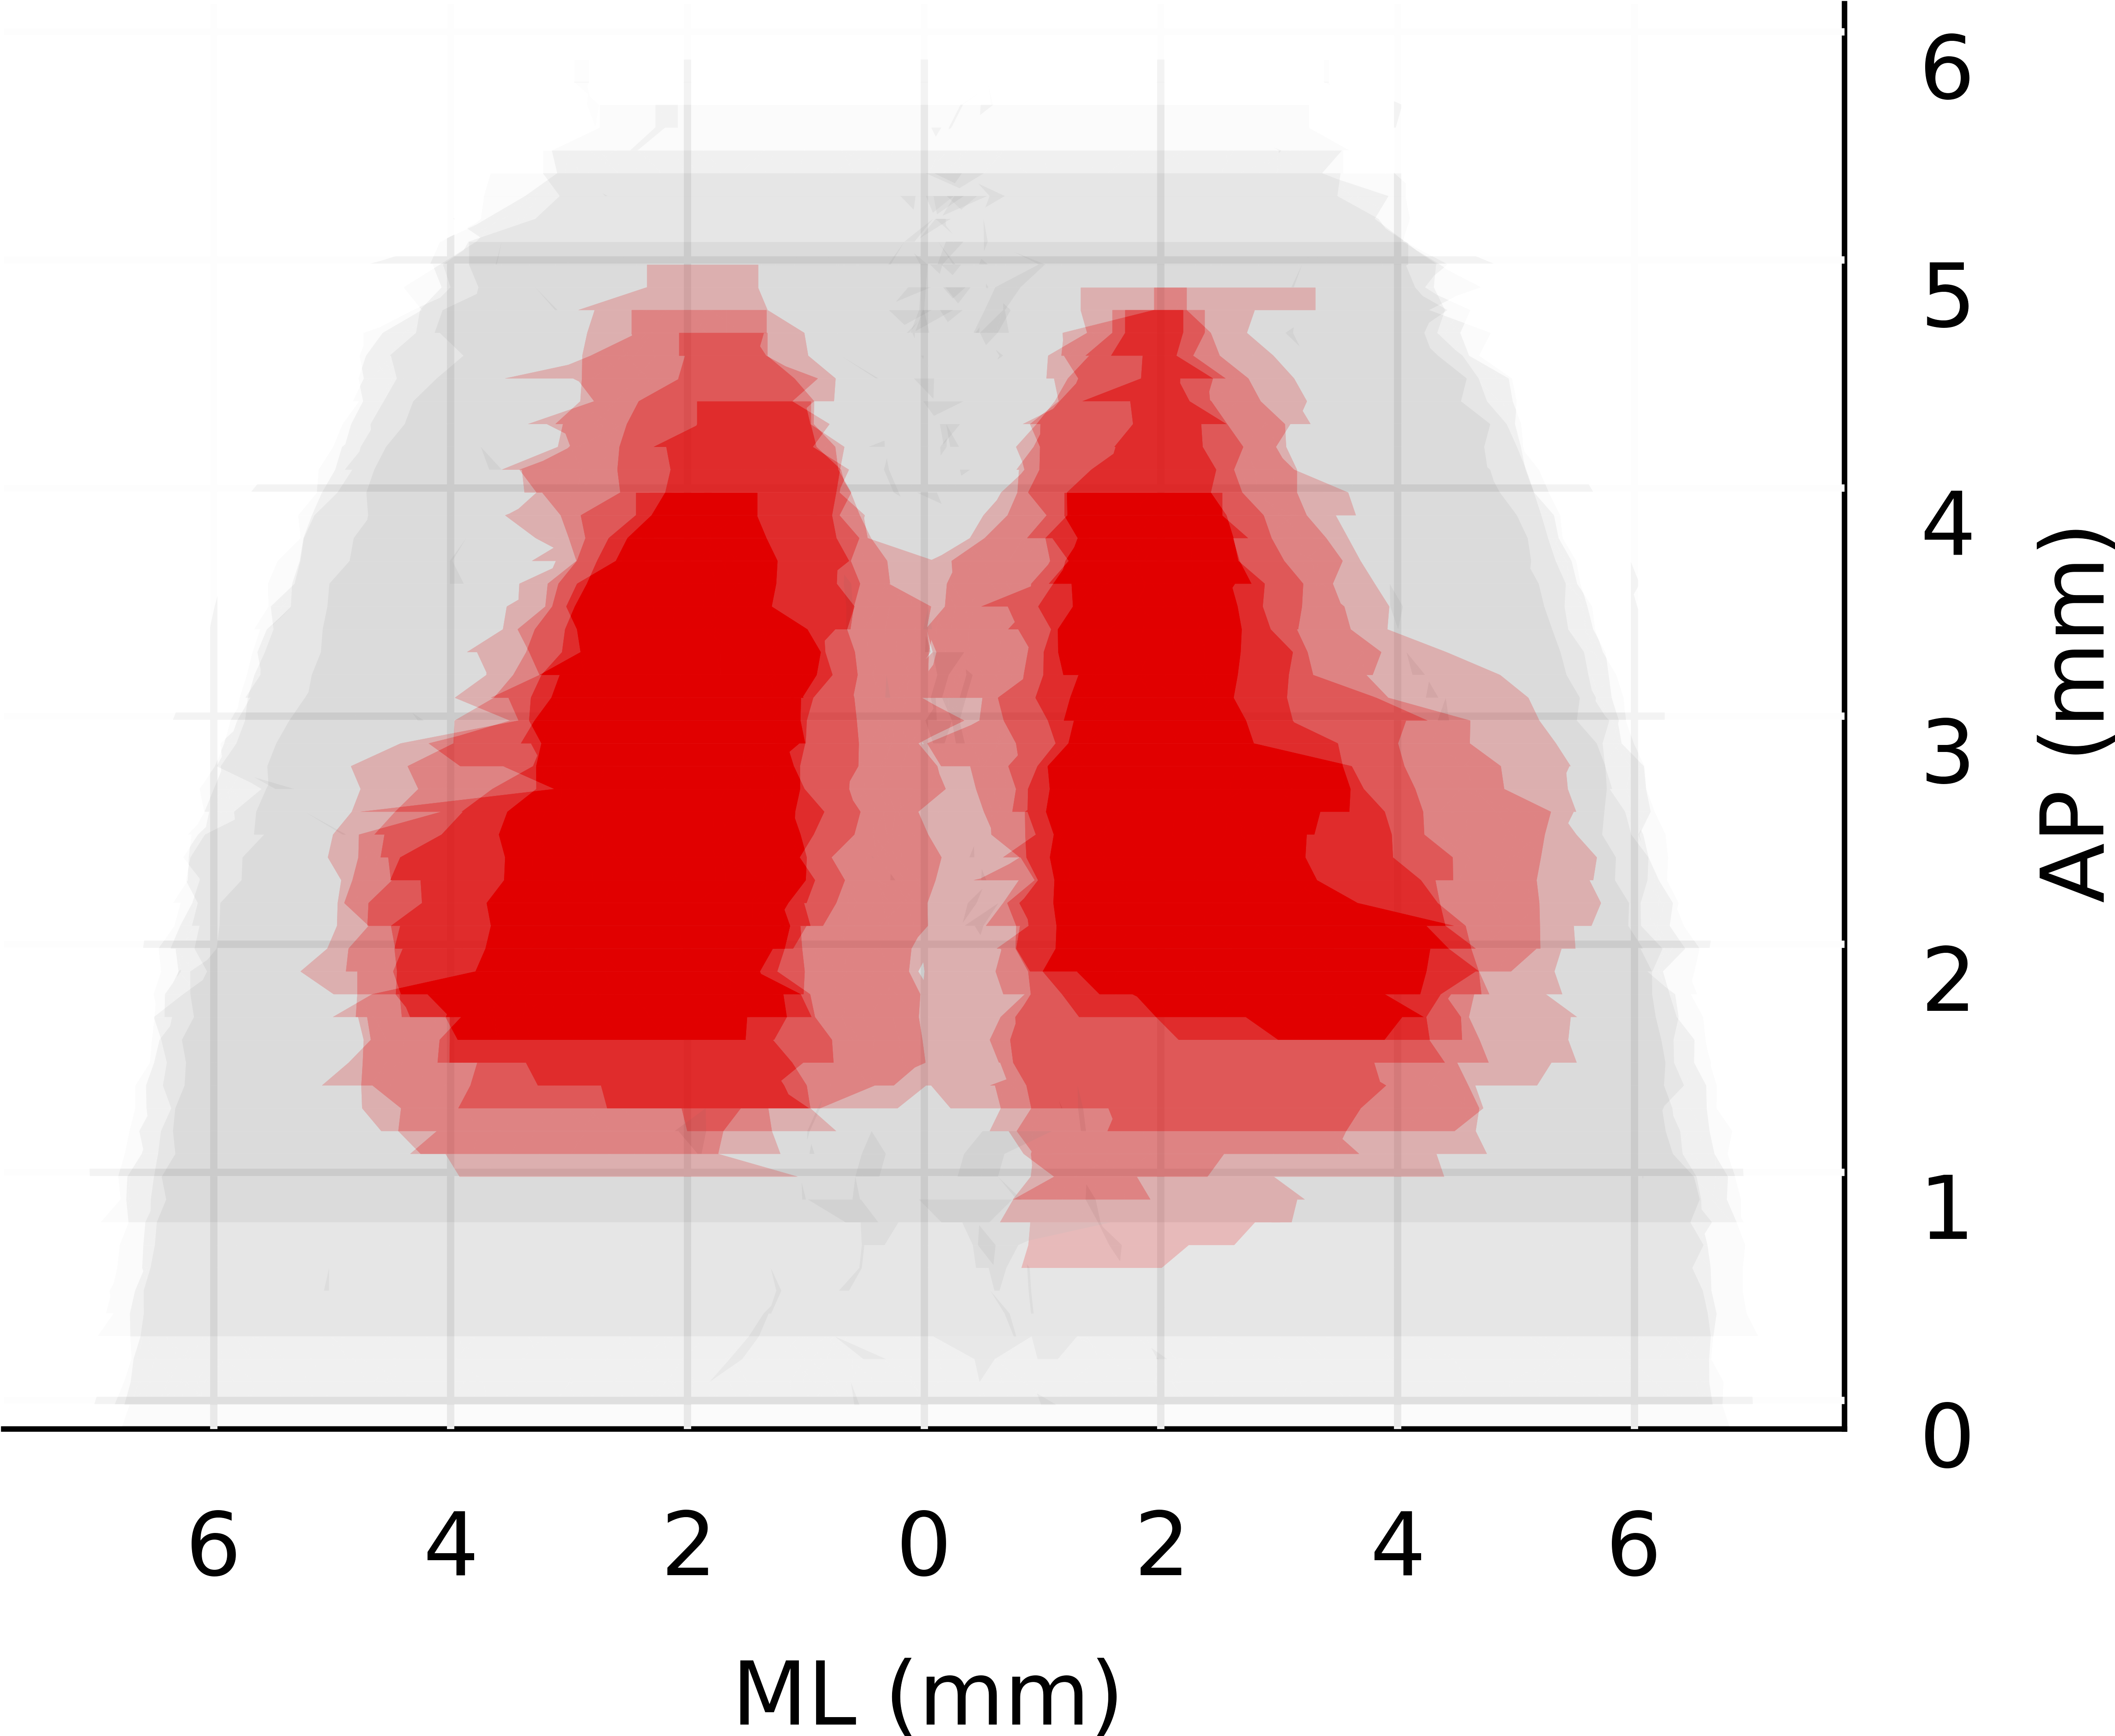
\includegraphics[width=0.5\textwidth]{elements/histology_large}};
  \node[draw=none,above=0mm of large] {large lesions (> \SI{15}{\milli\meter\cubed})};
  \node[draw=none,above left=5mm and 0mm of large] {D};
\end{tikzpicture}
\end{document}